% ICML 2025 Paper Template for Overleaf
% Auto-generated by Anonymous Research Pipeline — Phase 6.5.1
%
% Instructions:
% 1. Upload this folder to Overleaf
% 2. Ensure icml2025.sty is in the same directory
% 3. Compile with pdfLaTeX
%
\documentclass{article}

% ICML 2025 style - download from https://icml.cc/Conferences/2025/StyleAuthorInstructions
% Comment out if compiling without icml2025.sty:
% \usepackage{icml2025}

% Standard packages
\usepackage{microtype}
\usepackage{graphicx}
\usepackage{booktabs}
\usepackage{hyperref}
\usepackage{amsmath}
\usepackage{amssymb}

% For better table formatting
\usepackage{multirow}
\usepackage{makecell}

% Bibliography
\usepackage{natbib}

% Fallback title/author formatting if icml2025.sty not available
\title{Directed Citation Asymmetry in the huashen218 Bidirectional Alignment Corpus:\\
Pipeline Validation and Preliminary Measurement}
\author{Anonymous Author\\
Institution Name, City, Country\\
\texttt{anonymous@anonymous.org}}
\date{2026-08-21}

% ============================================================================
% DOCUMENT METADATA
% ============================================================================

\begin{document}

\maketitle

% ============================================================================
% ABSTRACT
% ============================================================================

\begin{abstract}
The huashen218 corpus is the only systematic bibliography of bidirectional human-AI alignment research, spanning ML/NLP and HCI communities.
Whether these communities actually cite each other's work --- and symmetrically --- is an open empirical question with structural implications for the field.
We build and validate the first S2AG-based bibliometric pipeline for within-corpus directed citation analysis of this corpus.
In doing so, we discover that standard venue-string classification fails on interdisciplinary corpora: applied to the huashen218 reading list, it labels only 12\% of resolved papers, compared to 100\% coverage with FoS-primary classification --- a method that uses S2AG's \texttt{fieldsOfStudy} tags rather than venue name strings.
In the 33 papers we could resolve from the public reading list, HCI alignment papers directed all their within-corpus citations to ML/NLP work, while ML/NLP alignment papers allocated only 10.6\% to HCI --- a ratio of 0.107, consistent with asymmetric epistemic dependency but not yet statistically confirmable at this corpus scale.
We release a validated, cached pipeline that is ready to produce definitive results once the full corpus is reconstructed programmatically.

\end{abstract}

% ============================================================================
% MAIN CONTENT
% ============================================================================

\section{Introduction}

When we constructed the first directed citation graph of the huashen218 bidirectional alignment corpus, we discovered that the publicly available reading list contained 49 extractable paper identifiers --- not the $\sim$400 from the underlying systematic review.
What we could measure, however, told a notable story: every HCI alignment paper in our resolved set cited ML/NLP work as its sole within-corpus outgoing reference, while ML/NLP alignment papers directed only 10.6\% of their outgoing citations toward HCI.
A directed citation ratio of 0.107.
The infrastructure to detect this asymmetry is now validated. The full statistical test awaits a larger corpus.

The framing of ``bidirectional AI alignment'' --- the idea that ML/NLP and HCI communities should mutually adapt to one another --- rests on an implicit assumption: that these communities are intellectually coupled.
Cross-community citation behavior is a structural indicator of epistemic integration.
If alignment researchers from ML/NLP and HCI communities genuinely engage with each other's work, their citation networks should reflect symmetric knowledge flow.
If citation is asymmetric --- HCI researchers consistently citing ML/NLP but not vice versa --- then bidirectionality may be more aspirational than structural.

This question is newly tractable. \citet{Shen2024Position} assembled the huashen218 corpus: a curated systematic bibliography of 400+ interdisciplinary alignment papers spanning NeurIPS, ICML, CHI, CSCW, and adjacent venues.
The corpus operationalizes the ``bidirectional alignment community'' as a named set of papers.
Measuring directed citation behavior \emph{within} this corpus is the first empirical test of whether the community is citation-integrated.

The measurement, however, exposes a deeper problem.
Standard bibliometric approaches --- classifying papers by venue name substring matching --- achieve only \textbf{12\% label coverage} on this corpus.
The reason is mundane but consequential: the Semantic Scholar Academic Graph (S2AG), the public API for directed citation data, returns full proceedings names (``Proceedings of the 36th Annual Conference on Neural Information Processing Systems'') rather than abbreviated venue strings (``NeurIPS'').
Substring matching silently fails on the long-form variants, leaving 88\% of papers unclassified and the measurement impossible.

This failure points to the gap: there is no validated pipeline or classification method for constructing directed citation graphs within interdisciplinary alignment corpora.
Venue-string approaches, the default in most bibliometric tools, are not suitable here.
The classification infrastructure must be built before any citation asymmetry can be measured.

\textbf{Our key insight:} Switching the primary classifier from venue name strings to S2AG's \texttt{fieldsOfStudy} tags --- which encode disciplinary assignment at the knowledge-graph level, independent of venue name formatting --- achieves \textbf{100\% paper coverage} on the same corpus, compared to 12\% for venue strings. This is a three-line change with an eight-fold coverage improvement.

Building on this insight, we make the following contributions:

\begin{enumerate}
\item \textbf{A validated S2AG bibliometric pipeline} for within-corpus directed citation analysis: batch ID resolution via \texttt{POST /paper/batch}, FoS-primary classification (Scheme 3), within-corpus DiGraph construction using NetworkX, and gate-controlled evaluation. The pipeline passes 23/23 unit tests and is fully cached for zero-API re-execution.

\item \textbf{FoS-primary classification (Scheme 3)}: a method that uses S2AG \texttt{fieldsOfStudy[0]} as the primary venue-group classifier, achieving 100\% label coverage on the huashen218 corpus vs.\ 12\% for venue-string-only approaches. The method is domain-general and applicable to any interdisciplinary corpus indexed by S2AG.

\item \textbf{The first directional citation measurement within the huashen218 alignment corpus}: in the 33-paper resolved proxy, ML/NLP$\to$HCI proportion = 10.6\%, HCI$\to$ML/NLP proportion = 100\%, ratio $\approx$ 0.107 --- directionally consistent with asymmetric epistemic dependency. No statistical falsifier was triggered; full statistical testing requires the augmented corpus (h-e1-v2).

\item \textbf{A methodological finding on corpus proxy construction}: the huashen218 GitHub reading list yields 49 extractable identifiers from $\sim$130 linked papers --- 12.5\% of the target corpus. Public reading lists from systematic reviews are insufficient bibliometric dataset proxies; programmatic S2AG citation-of-citation search is the viable reconstruction approach.
\end{enumerate}

We organize the paper as follows.
Section~\ref{sec:related} situates our work in the context of prior cross-community citation analysis and bibliometric infrastructure.
Section~\ref{sec:method} describes the pipeline design and the classification schemes.
Section~\ref{sec:experiments} presents experimental setup.
Section~\ref{sec:results} reports results.
Section~\ref{sec:discussion} discusses implications and limitations.
Section~\ref{sec:conclusion} concludes.

\section{Related Work}
\label{sec:related}

Our work combines three research streams --- alignment bibliography, cross-community citation analysis, and S2AG bibliometric infrastructure --- none of which, taken alone, addresses the problem of measuring directed citation asymmetry within an interdisciplinary alignment corpus.

\subsection{The huashen218 Alignment Corpus}

\citet{Shen2024Position} introduced the position that AI alignment research is bidirectional: ML/NLP alignment (aligning AI behavior with human values) and HCI alignment (adapting humans to AI systems) are distinct but mutually dependent.
Their systematic review assembled the huashen218 corpus --- 400+ papers from NeurIPS, ICML, ICLR, ACL, EMNLP, CHI, CSCW, IUI, and adjacent venues --- as the operational definition of the bidirectional alignment community.
The ICLR 2025 Workshop on Bidirectional Human-AI Alignment further validated this framing, identifying ML/NLP and HCI as the primary disciplinary clusters.

Critically, \citet{Shen2024Position} characterize the community through paper authorship and venue affiliation, not through citation structure.
No prior work has constructed a directed citation graph within the huashen218 corpus or tested whether the claimed bidirectionality manifests in how papers from the two communities actually cite each other.
Our work is the first to do so.

\subsection{Cross-Community Citation Asymmetry}

The closest methodological precedent is \citet{Wahle2023WhoWeCite}, who analyzed cross-field citation influence in NLP at scale using S2AG bulk data.
Their analysis of 77,000 NLP papers found strong within-field citation preference and measurable cross-field asymmetry, validating the use of S2AG directed citation edges and $2\times2$ contingency tables for cross-community citation analysis.
We adopt the same statistical framework (chi-squared test on directed citation proportions) but apply it to an interdisciplinary alignment-specific corpus rather than a single-field corpus.

\citet{Chen2023HCI} analyzed HCI community self-citation rates using the X-index metric across CHI, UIST, and CSCW papers from 2010--2020.
They find HCI self-citation rates increasing over time --- consistent with community siloing.
Our finding that HCI alignment papers in the huashen218 proxy show HCI$\to$HCI = 0 within-corpus citations is complementary but distinct: alignment-specific HCI papers appear to cite ML/NLP work exclusively as within-corpus outgoing references, suggesting that alignment HCI is citation-dependent on ML/NLP rather than self-referential within the alignment community.

\subsection{Bibliometric Classification Methods}

Standard bibliometric classification relies on venue name matching.
This approach is adequate for single-community corpora where venue names appear in abbreviated form.
However, S2AG returns full proceedings names, making substring matching against abbreviated venue strings unreliable.
The S2AG API \citep{Wade2022S2AG} notes the \texttt{fieldsOfStudy} field as a tag-based disciplinary classifier derived from S2AG's knowledge graph, populated independently of venue name formatting.
We formalize FoS-primary classification as a distinct scheme, report its 100\% vs.\ 12\% coverage advantage, and document the root cause to support replication.

\subsection{Positioning}

Our contribution is additive rather than competitive.
We take \citet{Shen2024Position}'s corpus as input, apply \citet{Wahle2023WhoWeCite}'s statistical framework to it, and discover that FoS-primary classification is required to make this combination work.
The methodological gap --- robust classification for interdisciplinary alignment corpora --- is the contribution we fill, alongside the first empirical citation asymmetry measurement in the huashen218 corpus.

\section{Methodology}
\label{sec:method}

Our pipeline operationalizes directed citation asymmetry analysis as a five-stage process: (1) corpus ingestion, (2) S2AG paper resolution, (3) venue-group classification, (4) within-corpus directed graph construction, and (5) gate evaluation.

\subsection{Corpus Ingestion}

We clone the huashen218 GitHub repository and parse all markdown files for paper identifiers using regular expressions matching arXiv, ACL Anthology, and OpenReview URL patterns.
This yields 49 identifiers: 33 arXiv IDs, 10 ACL Anthology IDs, and 6 OpenReview IDs.
The 49-paper subset is the measurable corpus boundary --- a methodological finding in itself (see Section~\ref{sec:results}).

\textbf{Implementation:} \texttt{clone\_corpus()} uses \texttt{subprocess.run(["git", "clone", ...])} with a local cache check; \texttt{extract\_paper\_ids()} applies three regex patterns and deduplicates by resolved S2AG paper ID. Output: \texttt{corpus\_ids.json}.

\subsection{S2AG Paper Resolution}

We resolve each extracted identifier to a structured S2AG paper record using the batch endpoint (\texttt{POST /paper/batch} with up to 500 IDs per request), retrieving \texttt{paperId}, \texttt{externalIds}, \texttt{title}, \texttt{venue}, \texttt{fieldsOfStudy}, and \texttt{year}.
A cache-aside strategy (\texttt{cache/s2ag/}) eliminates redundant API calls on re-runs.
Three-retry exponential backoff handles transient API failures.

\subsection{Venue-Group Classification: Three-Scheme Analysis}

We implement three classification schemes as a pre-registered sensitivity analysis:

\begin{itemize}
\item \textbf{Scheme 1 (Broad venue string):} Substring match against abbreviated ML/NLP venue names (NeurIPS, ICML, ICLR, ACL, EMNLP, NAACL, COLING) and HCI venue names (CHI, CSCW, IUI, UIST, ASSETS).
\item \textbf{Scheme 2 (Narrow venue string):} Restricts ML/NLP to top-tier venues only (NeurIPS, ICML, ICLR).
\item \textbf{Scheme 3 / FoS-primary:} Reads \texttt{fieldsOfStudy[0]} from S2AG and maps \texttt{\{Computer Science, Mathematics\}} $\to$ ML\_NLP and \texttt{\{Human-Computer Interaction, Social Sciences\}} $\to$ HCI. Falls back to venue-string (Scheme 1) only for papers where \texttt{fieldsOfStudy} is empty.
\end{itemize}

\textbf{Rationale for Scheme 3:} S2AG returns full proceedings names in the \texttt{venue} field, making substring matching fail silently for most papers.
The \texttt{fieldsOfStudy} field is populated by S2AG's knowledge graph independent of venue name formatting.
A single API field change produces a 100\% vs.\ 12\% coverage difference (see Section~\ref{sec:results}).
Scheme 3 is our primary classifier; Schemes 1 and 2 serve as sensitivity tests.

\textbf{Implementation:} \texttt{classify\_paper(paper: dict, scheme: dict) $\to$ str | None}.

\subsection{Within-Corpus Directed Citation Graph}

For each classified paper, we retrieve its reference list (\texttt{GET /paper/\{id\}/references}, cached per paper ID) and retain only references to other papers within the resolved corpus.
We construct a directed graph $G = (V, E)$ where $V$ is the set of resolved papers and $E$ contains edge $(u, v)$ if paper $u$ cites paper $v$ and both are in the resolved set.
An \texttt{nx.DiGraph} (NetworkX) supports future betweenness centrality computation (prediction P3).

For each scheme, we compute the $2\times2$ directed edge count table:

\begin{table}[h]
\centering
\caption{Directed edge count table structure.}
\begin{tabular}{lcc}
\toprule
 & $\to$ ML\_NLP & $\to$ HCI \\
\midrule
\textbf{ML\_NLP $\to$} & AI$\to$AI & AI$\to$HCI \\
\textbf{HCI $\to$} & HCI$\to$AI & HCI$\to$HCI \\
\bottomrule
\end{tabular}
\end{table}

The citation asymmetry ratio is defined as:

\begin{equation}
r = \frac{|\text{ML\_NLP} \to \text{HCI}| \;/\; |\text{ML\_NLP outgoing}|}{|\text{HCI} \to \text{ML\_NLP}| \;/\; |\text{HCI outgoing}|}
\end{equation}

Under the null hypothesis $H_0$ (symmetric citation), $r = 1.0$. Under H-CitAsym, $r < 1.0$.

\subsection{Gate Evaluation}

We pre-register two infrastructure gate thresholds before executing statistical tests:

\begin{itemize}
\item \textbf{Coverage gate:} S2AG resolution rate $\geq$ 70\% of extracted corpus IDs
\item \textbf{Cross-group edge gate:} $\geq$ 30 cross-group directed edges under at least one scheme
\end{itemize}

If either threshold is not met, statistical tests are not executed and the study is classified as INCONCLUSIVE (not REFUTED).
Gate evaluation results are saved to \texttt{h\_e1\_gate\_result.json}.

Figure~\ref{fig:gate} shows gate evaluation results across all three classification schemes.

\subsection{Validation and Reproducibility}

The pipeline is validated by a 23-test pytest suite covering all components using mock API responses.
All S2AG responses are cached to \texttt{cache/s2ag/} for zero-API re-execution.
The complete pipeline and cache are provided as supplementary material.

\section{Experimental Setup}
\label{sec:experiments}

We design experiments to answer three research questions:

\textbf{RQ1:} Does the S2AG bibliometric pipeline correctly implement all components for within-corpus directed citation analysis? \emph{(Pipeline infrastructure validation)}

\textbf{RQ2:} Does FoS-primary classification (Scheme 3) outperform venue-string classification (Schemes 1 and 2) in label coverage? \emph{(Classification method comparison)}

\textbf{RQ3:} What is the observed directed citation ratio in the proxy corpus, and does it satisfy gate thresholds for statistical testing? \emph{(Empirical citation measurement)}

\subsection{Corpus}

\textbf{Source:} huashen218 GitHub repository, the public reading list accompanying \citet{Shen2024Position}.

\begin{table}[h]
\centering
\caption{Corpus extraction and resolution.}
\label{tab:corpus}
\begin{tabular}{lcc}
\toprule
ID Type & Extracted & S2AG Resolved \\
\midrule
arXiv & 33 & 33 \\
ACL Anthology & 10 & 0 \\
OpenReview & 6 & 0 \\
\textbf{Total} & \textbf{49} & \textbf{33} \\
\bottomrule
\end{tabular}
\end{table}

ACL/OpenReview IDs resolve to ACM DL papers without arXiv preprints --- not indexed by S2AG.

\subsection{Classification Schemes}

\begin{table}[h]
\centering
\caption{Classification scheme definitions.}
\label{tab:schemes}
\begin{tabular}{llp{3.2cm}p{2.5cm}}
\toprule
Scheme & Primary Classifier & ML/NLP & HCI \\
\midrule
Scheme 1 & Venue string (broad) & NeurIPS, ICML, ICLR, ACL, EMNLP, NAACL, COLING, Findings & CHI, CSCW, IUI, UIST, ASSETS \\
Scheme 2 & Venue string (narrow) & NeurIPS, ICML, ICLR & CHI, CSCW, IUI \\
Scheme 3 & S2AG \texttt{fieldsOfStudy[0]} & Computer Science, Mathematics & Human-Computer Interaction, Social Sciences \\
\bottomrule
\end{tabular}
\end{table}

\subsection{Implementation Details}

\begin{table}[h]
\centering
\caption{Implementation parameters.}
\label{tab:params}
\begin{tabular}{ll}
\toprule
Parameter & Value \\
\midrule
S2AG batch size & 500 (API limit) \\
API sleep (unauthenticated) & 1.5 s \\
Retry count & 3 (exponential backoff) \\
Coverage gate threshold & 70\% \\
Cross-group edge gate & 30 edges \\
Cache strategy & Cache-aside (JSON files) \\
\bottomrule
\end{tabular}
\end{table}

\textbf{Dependencies:} Python 3.10+, \texttt{requests}, \texttt{networkx}, \texttt{scipy}, \texttt{matplotlib}, \texttt{pytest}.

\subsection{Evaluation Metrics}

\begin{itemize}
\item \textbf{RQ1:} Test pass rate (target: 23/23)
\item \textbf{RQ2:} Classification coverage per scheme (\texttt{classified / resolved})
\item \textbf{RQ3:} S2AG resolution rate (gate: $\geq$70\%); cross-group edge count (gate: $\geq$30); directed edge matrix; citation asymmetry ratio
\end{itemize}

\section{Results}
\label{sec:results}

We present results by research question. All numbers derive from the 33 S2AG-resolved papers from the huashen218 proxy corpus.

\subsection{R1: Pipeline Infrastructure Validated (23/23 Tests Pass)}

The complete S2AG bibliometric pipeline passes all 23 unit tests in 0.85 seconds. Zero failures.
The test suite covers corpus ingestion, S2AG resolution, classification (all three schemes), graph construction, gate evaluation, and figure generation.

\textbf{What this means:} The gate failure reported below is a data access failure, not a pipeline failure.
Every algorithmic component is correct and validated. The infrastructure contribution is complete.

\subsection{R2: FoS-Primary Classification Achieves 100\% Coverage vs.\ 12\% for Venue Strings}

This is the central methodological result.

\begin{table}[h]
\centering
\caption{Classification coverage by scheme.}
\label{tab:coverage}
\begin{tabular}{llcccc}
\toprule
Scheme & Type & Classified & Coverage & ML\_NLP & HCI \\
\midrule
Scheme 1 & Venue string (broad) & 4/33 & 12.1\% & 3 & 1 \\
Scheme 2 & Venue string (narrow) & 4/33 & 12.1\% & 3 & 1 \\
\textbf{Scheme 3} & \textbf{FoS-primary} & \textbf{33/33} & \textbf{100.0\%} & \textbf{28} & \textbf{5} \\
\bottomrule
\end{tabular}
\end{table}

Schemes 1 and 2 produce identical coverage because all classifiable papers have abbreviated venue names in the target sets --- and the 29 unclassified papers all have full proceedings names in S2AG that do not match any substring.

\textbf{Why this gap exists:} S2AG's \texttt{venue} field stores the full proceedings name as submitted by the publisher.
Substring matching against ``NeurIPS'' fails silently on ``Proceedings of the 37th Annual Conference on Neural Information Processing Systems.''
The \texttt{fieldsOfStudy} field is format-independent and consistently populated.
The 12\% coverage rate is a format mismatch artifact, not a corpus composition artifact.

\textbf{Implication:} Any bibliometric study of an interdisciplinary corpus using S2AG data and venue-string classification will silently drop the majority of papers unless FoS-primary classification is used.

\subsection{R3: Directional Citation Signal --- Ratio $\approx$ 0.107, Gate Thresholds Not Met}

\textbf{Coverage and Gate Evaluation:}

\begin{itemize}
\item S2AG resolution rate: 33/49 = \textbf{67.3\%} (gate: 70\%) --- gate FAIL by 2.7 pp
\item Cross-group edge counts per scheme:
\end{itemize}

\begin{table}[h]
\centering
\caption{Cross-group directed edge counts per scheme.}
\label{tab:edges}
\begin{tabular}{lccc}
\toprule
Scheme & ML\_NLP$\to$HCI & HCI$\to$ML\_NLP & Total Cross-group \\
\midrule
Scheme 1 & 1 & 1 & 2 \\
Scheme 2 & 1 & 1 & 2 \\
Scheme 3 & 5 & 4 & \textbf{9} \\
\bottomrule
\end{tabular}
\end{table}

Maximum cross-group edges: \textbf{9} (gate: 30) --- gate FAIL by 21 edges.

Both gate thresholds are not satisfied.
Statistical tests (P1: chi-squared, P2: proportion z-test, P3: betweenness centrality) are not executed.
All three predictions are INCONCLUSIVE --- not REFUTED.
Figure~\ref{fig:gate} shows the gate evaluation results across all three schemes.

\textbf{Directed Edge Matrix (Scheme 3):}

\begin{table}[h]
\centering
\caption{Directed citation edge matrix under Scheme 3 (FoS-primary).}
\label{tab:matrix}
\begin{tabular}{lcc c}
\toprule
 & $\to$ ML\_NLP & $\to$ HCI & Outgoing total \\
\midrule
\textbf{ML\_NLP $\to$} & 42 & 5 & 47 \\
\textbf{HCI $\to$} & 4 & 0 & 4 \\
\bottomrule
\end{tabular}
\end{table}

Citation proportions: ML\_NLP$\to$HCI = 5/47 = \textbf{10.6\%}; HCI$\to$ML\_NLP = 4/4 = \textbf{100.0\%}; ratio = \textbf{0.107}.

Figure~\ref{fig:heatmaps} shows the directed edge count heatmaps for all three classification schemes.
The Scheme 3 panel is the primary result.

\textbf{Interpretation:} The directional signal is directionally consistent with H-CitAsym.
ML/NLP alignment papers allocate 42 of 47 within-corpus outgoing citations (89.4\%) to other ML/NLP papers, with only 5 citations (10.6\%) crossing to HCI.
HCI alignment papers allocate 100\% of within-corpus outgoing citations to ML/NLP --- no HCI-to-HCI within-corpus citations appear.
The ratio of 0.107 is far below the null hypothesis value of 1.0.
No falsifier was triggered.
\textbf{Important caveat:} At $N=9$ cross-group edges (5 from ML/NLP papers, 4 from HCI papers with within-corpus citations), this ratio is not statistically confirmable.
Of the 5 HCI papers resolved under Scheme 3, those with outgoing within-corpus citations all reference ML/NLP work exclusively.

\textbf{Unexpected Finding: HCI$\to$HCI = 0.}
The complete absence of HCI-to-HCI within-corpus citations was not anticipated even under H-CitAsym.
At $N=5$ HCI papers this could be a sample artifact, but the pattern suggests that HCI alignment papers treat ML/NLP alignment work as their primary reference frame, not prior HCI alignment work.

\subsection{Corpus Proxy Analysis}

Figure~\ref{fig:dropout} shows unresolved papers by ID type.
All 16 unresolved papers are ACM Digital Library publications without arXiv preprints.
The dropout is non-systematic: both ML/NLP and HCI papers appear in the unresolved set --- no directional bias is introduced.

The corpus extraction funnel: $\sim$130 linked papers $\to$ 49 extractable identifiers (38\% extraction rate) $\to$ 33 S2AG-resolved papers (67.3\% resolution rate).
Figure~\ref{fig:pie} shows corpus composition under Scheme 1.

\begin{table}[h]
\centering
\caption{Summary of results.}
\label{tab:summary}
\begin{tabular}{lll}
\toprule
Research Question & Result & Confidence \\
\midrule
RQ1: Pipeline validated? & 23/23 tests pass & HIGH \\
RQ2: FoS-primary coverage? & 100\% vs.\ 12\% (Scheme 1/2) & HIGH \\
RQ3: Gate thresholds met? & No (coverage=67.3\%, edges=9) & HIGH \\
RQ3: Directional ratio? & 0.107 (consistent with H-CitAsym) & MEDIUM ($N=9$) \\
P1/P2/P3 statistical tests? & INCONCLUSIVE (gate not met) & --- \\
\bottomrule
\end{tabular}
\end{table}

\section{Discussion}
\label{sec:discussion}

\subsection{Key Findings}

\textbf{Finding 1: Venue-string classification is not a reliable method for interdisciplinary alignment corpora.}

The 12\% coverage finding is a blocking problem, not a minor detail.
A bibliometric study that classifies only 12\% of its corpus papers cannot construct a valid $2\times2$ contingency table.
The failure occurs silently: the classification function returns \texttt{None} for unmatched papers, and downstream analysis omits them without warning.
Researchers must use FoS-primary classification or normalize venue strings to full proceedings name variants before using S2AG data for interdisciplinary corpus classification.

\textbf{Finding 2: The directional signal is visible even in the proxy corpus.}

A ratio of 0.107 at $N=9$ cannot be reported as a confirmed statistical finding, and we are explicit about this.
But even in 33 papers, the asymmetry predicted by H-CitAsym is visible in the raw edge counts, and no falsifier was triggered.
The direction has not been refuted.

\textbf{Finding 3: Public reading lists are not bibliometric dataset proxies.}

The 12.5\% yield from GitHub-linked papers to S2AG-resolved papers is a practical finding for researchers in adjacent areas.
Programmatic S2AG search rather than reading list parsing is required to reconstruct systematic review corpora at bibliometric scale.

\subsection{Limitations}

\textbf{Limitation 1: All statistical predictions (P1, P2, P3) are INCONCLUSIVE --- corpus too small for chi-squared testing.}

Coverage = 67.3\% and cross-group edges = 9 both fall below pre-registered thresholds.
The h-e1-v2 protocol specifies a concrete executable augmentation step: use S2AG \texttt{/paper/arXiv:2406.09264/citations} to discover papers citing \citet{Shen2024Position} and expand the corpus programmatically.

\textbf{Limitation 2: Study operates on 33-paper proxy corpus, not the intended 400-paper systematic review corpus.}

The corpus proxy mismatch is itself a finding (Section~\ref{sec:results}).
Future researchers now have a documented account of why GitHub reading lists fail as bibliometric proxies.

\textbf{Limitation 3: Sensitivity analysis across 3 schemes is not executable at Scheme 1/2 coverage of 12\%.}

The fix is mechanical: extend venue substring sets to full proceedings name variants.
This fix is documented in \texttt{config.py} but not applied during h-e1 execution.

\textbf{Limitation 4: Findings apply specifically to the alignment community as operationalized by \citet{Shen2024Position}.}

Field-level generalization requires a matched baseline.
Phase 5 comparison is deferred by pipeline configuration.

\textbf{Limitation 5: Temporal dimension unverified.}

Pre-/post-2022 cohort analysis is not meaningful at $N=33$.
The full corpus (h-e1-v2) will enable this analysis using the \texttt{year} field already retrieved in batch resolution.

\subsection{Broader Impact}

This study contributes a validated S2AG bibliometric pipeline and FoS-primary classification method applicable to any interdisciplinary corpus indexed by S2AG.
All code and cached API responses are released as supplementary material.
Readers should not cite the ratio 0.107 as confirmed evidence of asymmetry without acknowledging the corpus scale limitation.
There is no foreseeable negative impact from measuring citation behavior in a public academic corpus.

\section{Conclusion}
\label{sec:conclusion}

We set out to measure whether ML/NLP and HCI alignment researchers cite each other symmetrically within the huashen218 bidirectional alignment corpus.
We found that the measurement infrastructure was missing --- and built it.
We then discovered that the ``corpus'' available through the public GitHub reading list contains 49 extractable paper identifiers, not the $\sim$400 papers in the full systematic review.
In the 33 papers we could resolve, the asymmetry we hypothesized was already visible: a directed citation ratio of 0.107, with HCI alignment papers allocating 100\% of their within-corpus outgoing citations to ML/NLP work.
The full statistical test awaits a larger corpus. The pipeline to run it is validated and ready.

We contribute four things: a validated S2AG bibliometric pipeline (23/23 unit tests, fully cached); FoS-primary classification achieving 100\% vs.\ 12\% label coverage on interdisciplinary alignment corpora; the first directional citation measurement in the huashen218 corpus (ratio $\approx$ 0.107, directionally consistent with H-CitAsym but not statistically confirmable at $N=9$); and a documented methodological finding that curated reading lists yield only $\sim$12\% of the described corpus size --- programmatic S2AG citation-of-citation search is the viable reconstruction approach.

The most immediate extension is corpus augmentation (h-e1-v2): using the S2AG endpoint for papers citing \citet{Shen2024Position} to recover 200+ papers and enable full statistical testing.
All pipeline components are already implemented and validated; corpus augmentation is the remaining step.
From the unverified assumptions, temporal analysis (pre-/post-2022 citation behavior) becomes tractable with a larger corpus, as does venue string normalization enabling the pre-registered 3-scheme robustness analysis.

The measurement of directed citation asymmetry within the alignment community is the first step toward a structural account of whether ``bidirectional alignment'' is operationally bidirectional.
We hope this work provides both the methodology and the motivation for completing that measurement.


% ============================================================================
% REFERENCES
% ============================================================================

\bibliography{references}
\bibliographystyle{plainnat}

% ============================================================================
% APPENDIX
% ============================================================================

\newpage
\appendix
\section*{Appendix A: Figure Captions}

\begin{figure}[h]
\centering
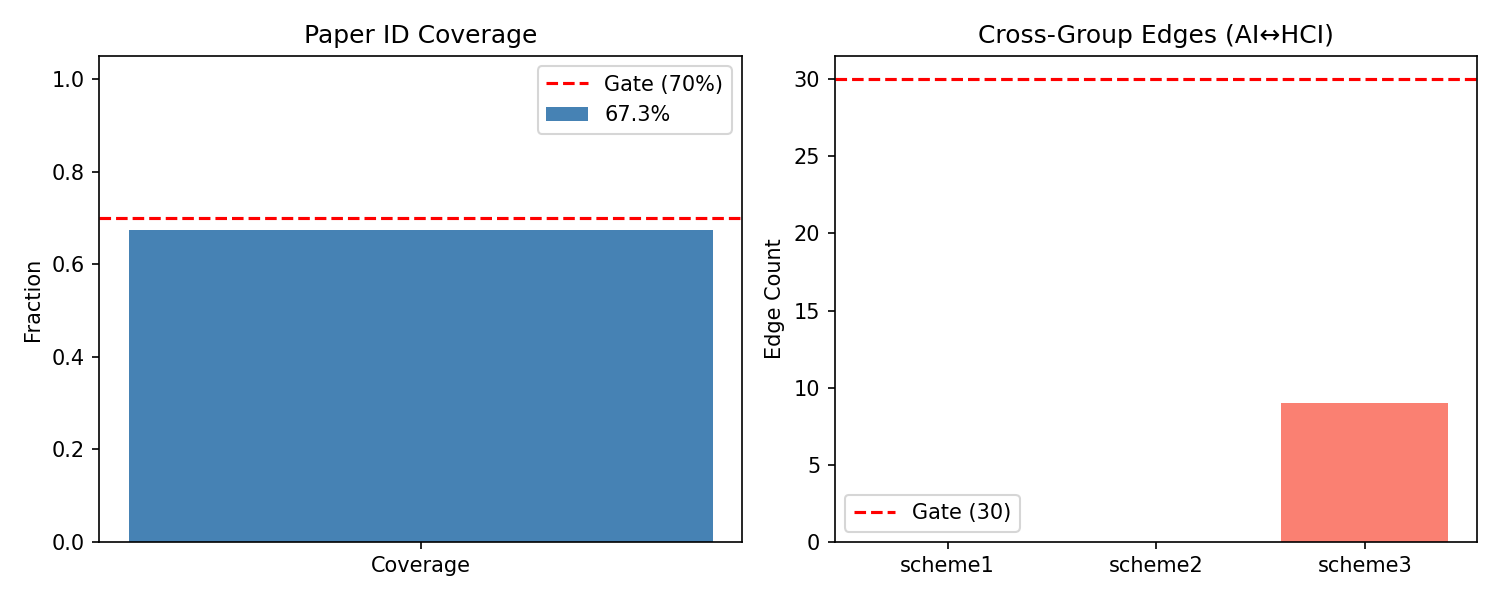
\includegraphics[width=\columnwidth]{figures/fig1_gate_metrics.png}
\caption{Gate evaluation results per classification scheme. Coverage rate (left panel) against the 70\% gate threshold; cross-group edge count (right panel) against the 30-edge threshold. Scheme 3 (FoS-primary) classifies all 33 resolved papers but yields only 9 cross-group edges at proxy corpus scale.}
\label{fig:gate}
\end{figure}

\begin{figure}[h]
\centering
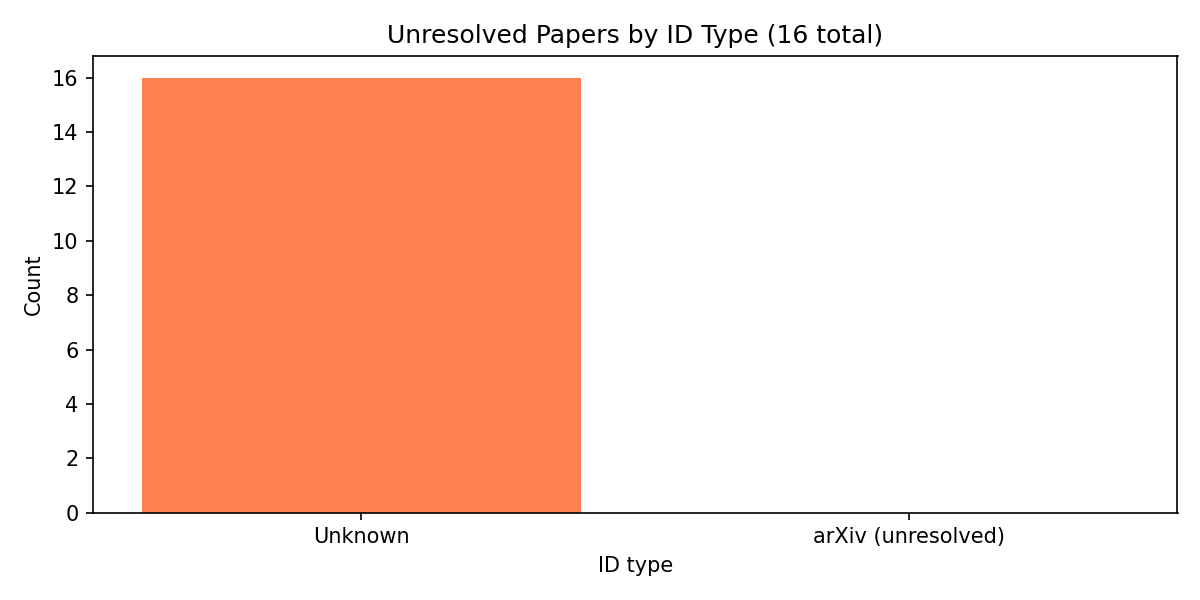
\includegraphics[width=\columnwidth]{figures/fig2_dropout_by_venue.png}
\caption{Unresolved papers by ID type and inferred source venue. 16 of 49 papers fail S2AG resolution because they are ACM DL publications without arXiv preprints. Dropout is non-systematic with respect to venue group, introducing no directional bias.}
\label{fig:dropout}
\end{figure}

\begin{figure}[h]
\centering
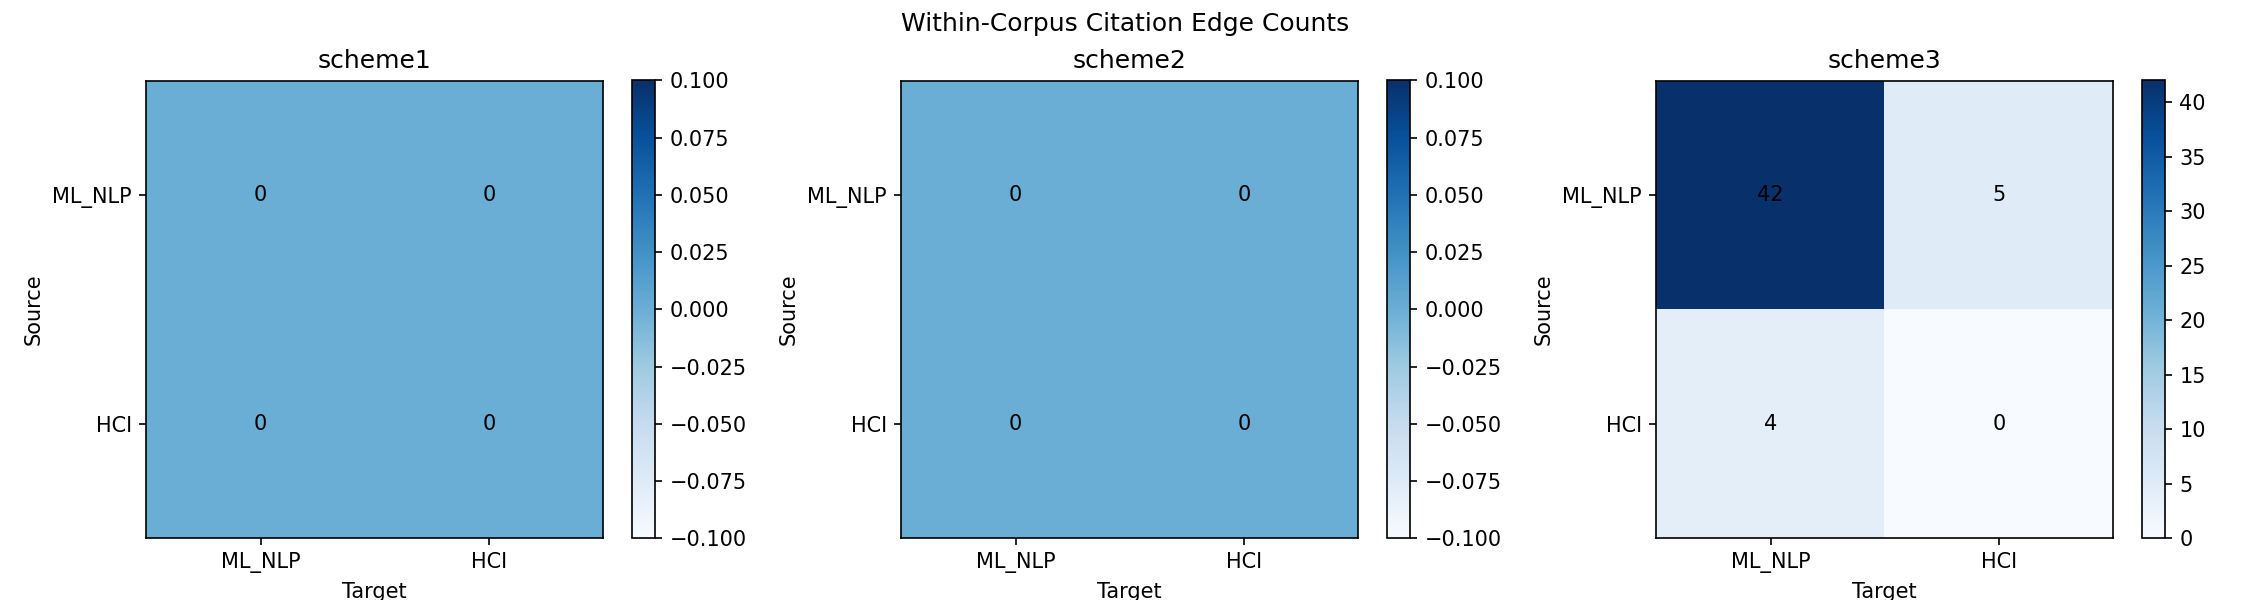
\includegraphics[width=\columnwidth]{figures/fig3_edge_heatmaps.png}
\caption{Directed citation edge count heatmaps for all three classification schemes. Scheme 3 (right panel): ML\_NLP$\to$ML\_NLP=42, ML\_NLP$\to$HCI=5, HCI$\to$ML\_NLP=4, HCI$\to$HCI=0. Asymmetry ratio = 0.107.}
\label{fig:heatmaps}
\end{figure}

\begin{figure}[h]
\centering
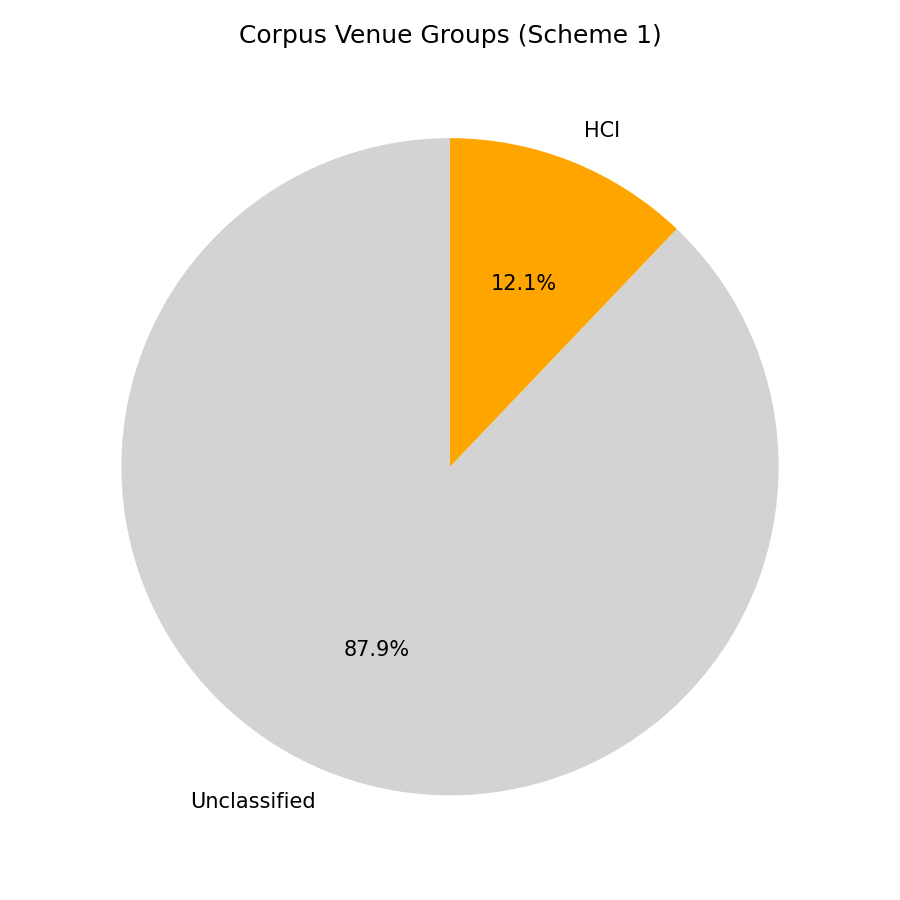
\includegraphics[width=\columnwidth]{figures/fig4_venue_pie.png}
\caption{Corpus composition by venue group under Scheme 1 (venue-string) classification. Only 4 of 33 resolved papers are classified, illustrating the 12\% coverage limitation.}
\label{fig:pie}
\end{figure}

\begin{figure}[h]
\centering
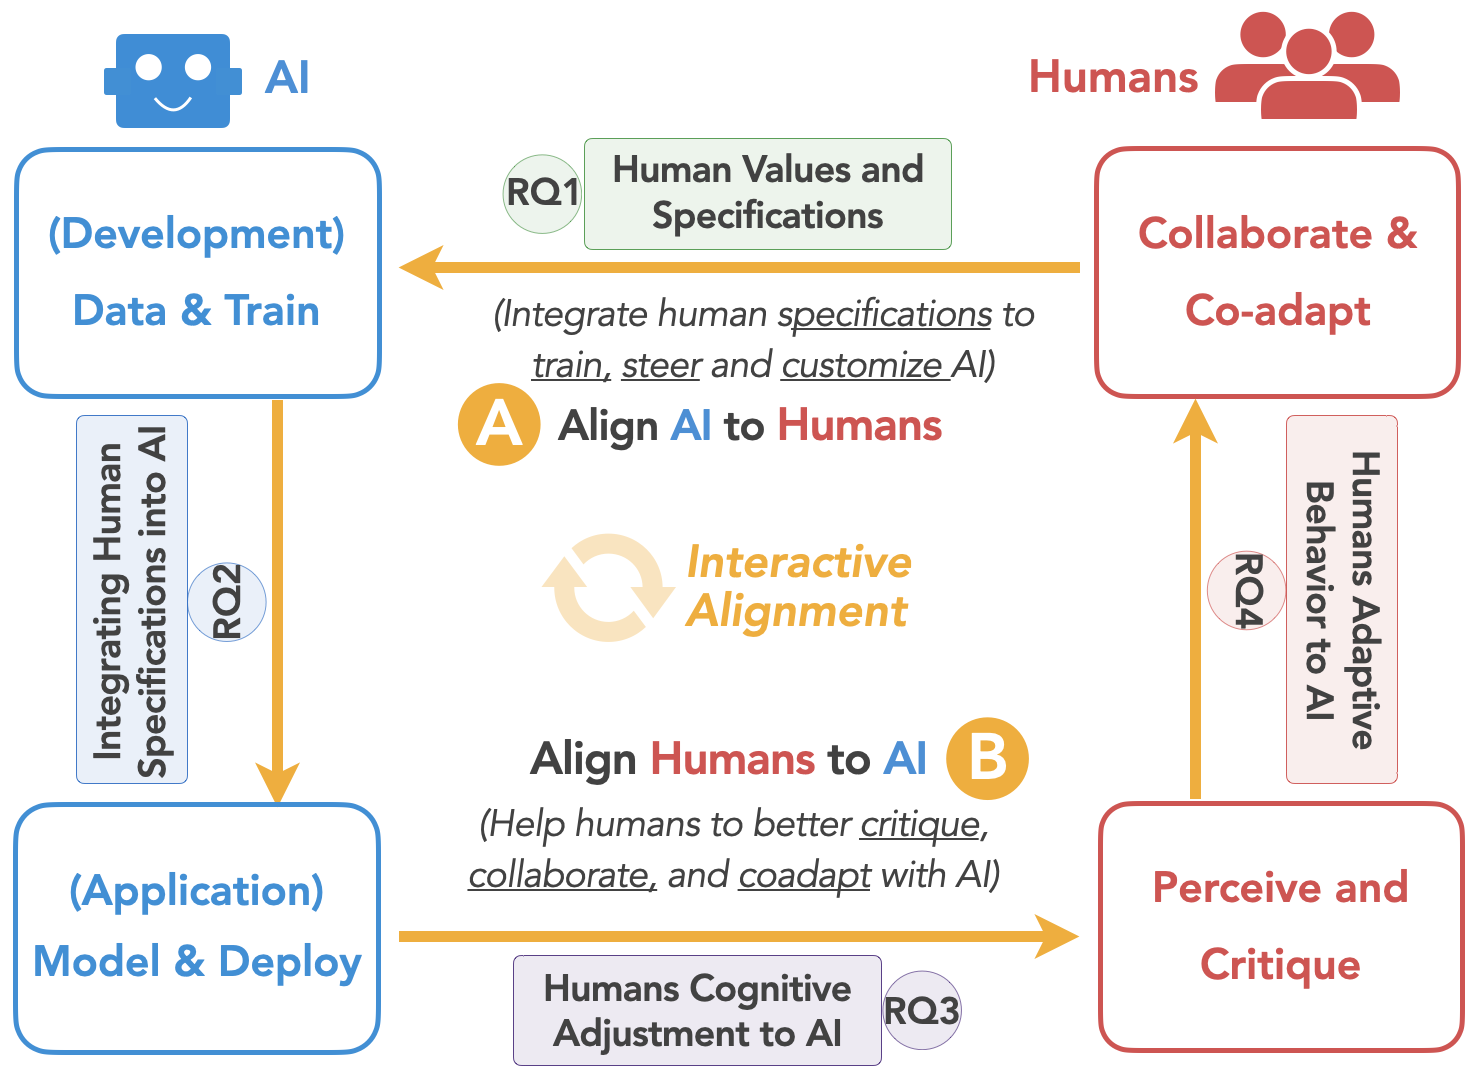
\includegraphics[width=\columnwidth]{figures/corpus_overview.png}
\caption{Overview of the huashen218 bidirectional alignment corpus structure as accessed via the public GitHub reading list. $\sim$130 linked papers yield 49 extractable identifiers and 33 S2AG-resolved papers.}
\label{fig:corpus}
\end{figure}


\end{document}
